\section{Introduction}

Scalable Internet architectures are typically composed of several specialized data systems. This is because web applications require a variety of data storage and query capabilities. Any single system is rarely a good fit to handle all the use-cases at scale while meeting the performance requirements. The most common data systems found in these architectures include relational databases, NoSQL data stores, caching engines and search indexes. Large scale social companies like LinkedIn will often build custom graph engines to handle complex graph queries at scale efficiently.

LinkedIn's data architecture consists of Oracle and MySQL as source-of-truth primary database technologies. There are a large number of specialized systems that have been built for serving complex use-cases like graph queries, search queries and ranking entities. Since reads outnumber writes by a large fraction in our workload, in many cases, we prefer to serve reads out of replica data stores; a technique commonly referred to as read-scaling. For example, there are cases when a single Oracle (running on expensive hardware) is the primary data store while many MySQL or Oracle instances (running on cheaper hardware) are serving reads. 
There are also other use-cases in the company that involve query result pre-computation, caching and near-line stream processing. 
There is therefore a need to capture all the changes that are happening to the primary databases and process it to populate the secondary data stores and indexes.
We also want to have a common data format that is both shared by all consumers and is independent of the source of truth. 
There are two ways we could have gone about building this. The first option is to write to the database and in parallel write to another messaging system. This is simple since the application code writing to the database is under our control. However it introduces a consistency problem because without a complex coordination protocol like Paxos~\cite{paxos} it is hard to ensure that both the database and the messaging system are in complete lock-step with each other in the face of failures. Both systems need to process exactly the same writes and need to serialize them in exactly the same order.
The second option is to make the database the source-of-truth, extract changes happening to the database and flow them through to the secondary data stores. This solves our consistency issue, but is challenging because databases like Oracle and MySQL have replication solutions that are proprietary. Since we want to process the data changes with application code and then write to secondary data stores, we need the replication system to be user-space and source-agnostic. This independence from the data source is especially important in growing companies, because it prevents technology lock-in and downstream consumers don't have to understand proprietary formats. 

After evaluating the pros and cons of the two approaches, we decided to pursue the second option in trying to achieve source-agnostic change data capture. 

%% Comments from Lin
%% The paragraph below needs a crisp list of strength/differentiators databus provides. Organize points in bullets will help.
%% Then we can have list of use cases, the longer, the more angels, the better.
  
We've built Databus which provides a common pipeline for transporting these change data capture (CDC) events from the primary databases to various applications. 
There are custom adaptors written for Oracle and MySQL which extract the changes happening in the database and convert them to a storage-neutral format. 
It is extremely easy to add support for other kinds of data sources as long as they provide a transaction log with some amount of rewindability.
These changes are then transported via a lossless tier while retaining the source consistency semantics to the final consumers. 
Databus allows consumers to fall behind indefinitely and still catchup while shielding the data source from abusive scan queries. 
The subscription API allows applications to subscribe to changes from one or more data sources, and filter based on the keys of the events.  
The Social Graph Index which serves all graph queries at LinkedIn, the People Search Index which powers all searches for members at LinkedIn and the various read replicas for our Member Profile data are all fed and kept consistent via Databus. 
\begin{figure}
\centering
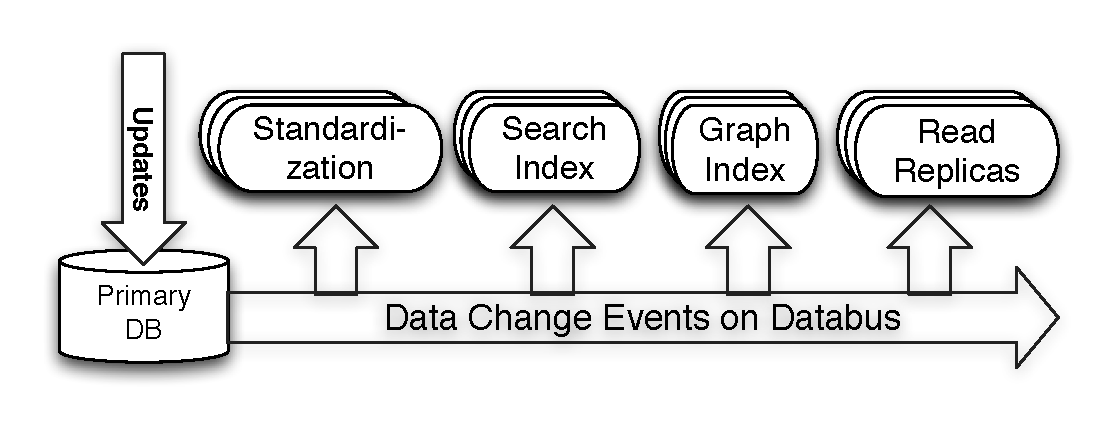
\epsfig{file=figures/databus-use-cases.eps, width=3in}
\caption{LinkedIn: Databus applications}
\label{fig:databus-use-cases}
\end{figure}





